\documentclass[tikz,border=8pt]{standalone}
\usepackage{tikz}
\usetikzlibrary{arrows.meta,calc}

\definecolor{primary}{HTML}{143264}
\definecolor{secondary}{HTML}{8C281E}
\definecolor{tealcol}{HTML}{117A65}
\definecolor{orangecol}{HTML}{C77C02}
\definecolor{greycol}{HTML}{505A64}

\begin{document}
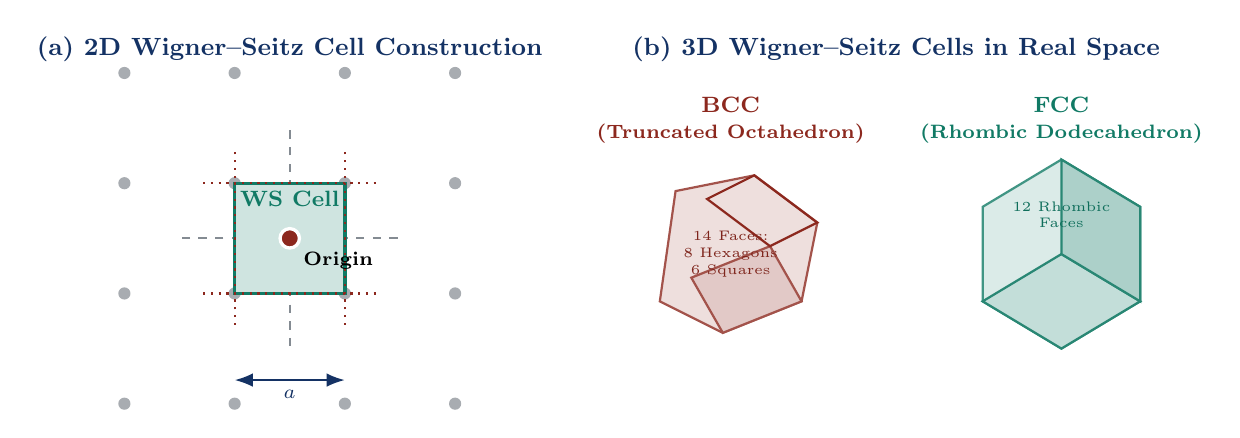
\begin{tikzpicture}[>=Latex]

  % Panel (a): 2D Wigner-Seitz Cell Construction
  \begin{scope}[shift={(0,0)}]
    \node[align=center, font=\bfseries\small, text=primary] at (2.1, 4.5) {(a) 2D Wigner--Seitz Cell Construction};
    
    \foreach \x in {0, 1.4, 2.8, 4.2} {
      \foreach \y in {0, 1.4, 2.8, 4.2} {
        \fill[greycol!50] (\x, \y) circle (2.2pt);
      }
    }
    
    \coordinate (C) at (2.1, 2.1);
    \coordinate (NN1) at (2.1, 3.5);
    \coordinate (NN2) at (3.5, 2.1);
    \coordinate (NN3) at (2.1, 0.7);
    \coordinate (NN4) at (0.7, 2.1);

    \draw[dashed, greycol!70, thick] (C) -- (NN1);
    \draw[dashed, greycol!70, thick] (C) -- (NN2);
    \draw[dashed, greycol!70, thick] (C) -- (NN3);
    \draw[dashed, greycol!70, thick] (C) -- (NN4);

    \fill[tealcol!20, draw=tealcol, very thick] 
      (1.4, 1.4) rectangle (2.8, 2.8);

    \draw[dotted, secondary, thick] (1.0, 2.8) -- (3.2, 2.8);
    \draw[dotted, secondary, thick] (2.8, 1.0) -- (2.8, 3.2);
    \draw[dotted, secondary, thick] (1.0, 1.4) -- (3.2, 1.4);
    \draw[dotted, secondary, thick] (1.4, 1.0) -- (1.4, 3.2);

    \filldraw[fill=secondary, draw=white, very thick] (C) circle (3.5pt) node[below right=1pt, font=\scriptsize\bfseries] {Origin};
    \node[font=\footnotesize\bfseries, tealcol] at (2.1, 2.1) [above=8pt] {WS Cell};
    \draw[<->, primary, thick] (1.4, 0.3) -- (2.8, 0.3) node[midway, below, font=\scriptsize] {$a$};
  \end{scope}

  % Panel (b): 3D Wigner-Seitz Cells of BCC and FCC
  \begin{scope}[shift={(6.2,0)}]
    \node[align=center, font=\bfseries\small, text=primary] at (3.6, 4.5) {(b) 3D Wigner--Seitz Cells in Real Space};

    % BCC WS Cell: Truncated Octahedron
    \begin{scope}[shift={(0,0.3)}]
      \node[align=center, font=\bfseries\footnotesize, text=secondary] at (1.5, 3.3) {BCC\\ \scriptsize (Truncated Octahedron)};
      \draw[thick, secondary!80, fill=secondary!15] 
        (0.6, 1.0) -- (1.4, 0.6) -- (2.4, 1.0) -- (2.6, 2.0) -- (1.8, 2.6) -- (0.8, 2.4) -- cycle;
      \draw[thick, secondary!80, fill=secondary!25] 
        (1.4, 0.6) -- (2.4, 1.0) -- (2.0, 1.7) -- (1.0, 1.3) -- cycle;
      \draw[thick, secondary] 
        (1.8, 2.6) -- (2.6, 2.0) -- (2.0, 1.7) -- (1.2, 2.3) -- cycle;
      \node[font=\tiny, text=secondary!90!black, align=center] at (1.5, 1.6) {14 Faces:\\8 Hexagons\\6 Squares};
    \end{scope}

    % FCC WS Cell: Rhombic Dodecahedron
    \begin{scope}[shift={(4.2,0.3)}]
      \node[align=center, font=\bfseries\footnotesize, text=tealcol] at (1.5, 3.3) {FCC\\ \scriptsize (Rhombic Dodecahedron)};
      \draw[thick, tealcol!80, fill=tealcol!15] 
        (1.5, 0.4) -- (2.5, 1.0) -- (2.5, 2.2) -- (1.5, 2.8) -- (0.5, 2.2) -- (0.5, 1.0) -- cycle;
      \draw[thick, tealcol!90, fill=tealcol!25]
        (1.5, 0.4) -- (2.5, 1.0) -- (1.5, 1.6) -- (0.5, 1.0) -- cycle;
      \draw[thick, tealcol!90, fill=tealcol!35]
        (1.5, 1.6) -- (2.5, 1.0) -- (2.5, 2.2) -- (1.5, 2.8) -- cycle;
      \node[font=\tiny, text=tealcol!90!black, align=center] at (1.5, 1.6) [above=6pt] {12 Rhombic\\Faces};
    \end{scope}

  \end{scope}

\end{tikzpicture}
\end{document}
